\scanpage{101}
% L1
\deleted{\unsure{Ens de schémas sur $k$|Pseudo-schémas sur $k$}}

% L2
\diagram{\begin{tikzcd}[ampersand replacement=\&,column sep=large]
(\text{Ens. schématiques }\unsure{\}}\,\text{sur }k)
\arrow[r,swap,"\text{\unsure{pl.|pl\textsuperscript{t}.} fidèle}"] \&
\underline{\operatorname{Hom}}((\text{Ens schém.}/k),(\text{Ens}))
\end{tikzcd}}

% L3
\diagram{\begin{tikzcd}[ampersand replacement=\&,column sep=small]
\& X \& \& \\
S\arrow[ur,dashed,"\unsure{i}"] \& \& S'\arrow[ul]\arrow[ll] \& S''\arrow[l,shift left=.55ex]\arrow[l,shift right=.55ex]
\end{tikzcd}}

% L4
\deleted{\uline{application surjective}} \qquad \uline{morphisme fid. plat}

% L5
\uline{Tout épimorphisme est un morphisme de descente}

% L6--9; braces group 1--4, square brackets group 1--2 and 3--4.
\[
\left\{\begin{array}{l}
\left[\begin{array}{ll}
1) & \text{Existence de }\varprojlim\text{ finies}\\
2) & \text{Existence du quotient par un \unsure{graphe|couple|groupoïde} d'équivalence}
\end{array}\right.\\[3pt]
\left[\begin{array}{ll}
3) & \text{Tout épim est effectif}\\
4) & \text{Tout épim est universel}
\end{array}\right.
\end{array}\right.
\]
\margin{[\unsure{d'où|donc|dans} ça marche pour \unsure{prégraphes|prégroupes|présystèmes|groupoïdes} d'équivalence\ldots]}
% slanted; a long curved stroke goes down the right edge to the question mark beside 4').

% L10
\deleted{5) Tout morphisme se factorise par un produit \unsure{du|dans} [\unsure{épim, un mono}]}

% L11; encircling and crossing strokes over the right branch.
\diagram{\begin{tikzcd}[ampersand replacement=\&,column sep=small,row sep=small,execute at end picture={\draw[thin] ($(\tikzcdmatrixname-1-2.west)+(-.15,0)$) .. controls +(0,.8) and +(0.7,.6) .. ($(\tikzcdmatrixname-1-5.east)+(.18,.06)$) .. controls +(.5,-1.0) and +(.3,-.4) .. ($(\tikzcdmatrixname-2-5.south)+(-.4,-.05)$) .. controls +(-1,.10) and +(0,-.50) .. cycle; \draw[thin] (\tikzcdmatrixname-1-3.east) .. controls +(0,-.5) and +(-.2,-.4) .. (\tikzcdmatrixname-1-4.south) .. controls +(.2,.8) and +(-.15,.5) .. (\tikzcdmatrixname-2-5.west) .. controls +(.6,.45) and +(-.5,.08) .. (\tikzcdmatrixname-2-5.east);}]
\deleted{\unsure{E}}\arrow[r] \& \deleted{\unsure{1}} \&
\deleted{X\times_Y X}\arrow[r,shift left=.55ex]\arrow[r,shift right=.55ex] \&
\deleted{X}\arrow[r]\arrow[dr] \& \deleted{Y}\\
\& \& \& \& \deleted{\unsure{Y'\mathrm{Im}|Y'/\mathrm{Im}|X/\mathrm{Rel}}}
\end{tikzcd}}

% L12--15
\[
\left\{\begin{array}{l}
\left[\begin{array}{ll}
1') & \text{Existence de }\varinjlim\text{ finies}\\
2') & \text{Existence du \unsure{coquotient|conoyau} par un \unsure{cographe|cocouple|couple} d'équivalence}
\end{array}\right.\\[3pt]
\left[\begin{array}{ll}
3') & \text{Tout. mon est effectif}\\
4') & \text{\unsure{Cochangement|Co-changement|Changement} de base dans un monomorphisme}
\end{array}\right.
\end{array}\right.
\]
\margin{?}

% L16
\uline{Axiome géométrique} \qquad $X\times\coprod Y_i\simeq\coprod_i X\times Y_i$

% L17--18
[\unsure{ou aussi|en somme} : changt de base commute aux sommes, -- donc aux $\uline{\lim}$ finies ???]

% L19
$R\to S$
\figure{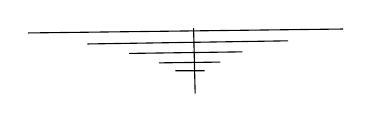
\begin{tikzpicture}[x=1cm,y=1cm]
\draw (-2,.40)--(2,.45) (-1.25,.26)--(1.30,.30) (-.72,.14)--(.72,.16) (-.34,.02)--(.44,.03) (-.13,-.08)--(.24,-.08) (.10,.46)--(.12,-.37);
\end{tikzpicture}}
% archive sheet number: 100
